%%%%%%%%%%%%%%%%%%%%%%%%%%%%%%%%%%%%%%%%%%%%%%%%
%% Intro to LaTeX and Template for Homework Assignments
%% Quantitative Methods in Political Science
%% University of Mannheim
%% Fall 2019
%%%%%%%%%%%%%%%%%%%%%%%%%%%%%%%%%%%%%%%%%%%%%%%%

% created by Marcel Neunhoeffer & Sebastian Sternberg


% This template and tutorial will help you to write up your homework. It will also help you to use Latex for other assignments than this course's homework.

%%%%%%%%%%%%%%%%%%%%%%%%%%%%%%%%%%%%%%%%%%%%%%%%
% Before we get started
%%%%%%%%%%%%%%%%%%%%%%%%%%%%%%%%%%%%%%%%%%%%%%%%

% Make an account on overleaf.com and get started. No need to install anything.

%%%%%%%%%%%%%%%%%%%%%%%%%%%%%%%%%%%%%%%%%%%%%%%%
% Or if you want it the nerdy way...
% INSTALL LATEX: Before we can get started you need to install LaTeX on your computer.
				% Windows: http://miktex.org/download
				% Mac:         http://www.tug.org/mactex/mactex-download.html	
				% There a many more different LaTeX editors out there for both operating systems. I use TeXworks because it looks the same on Windows and Mac.
				

% SAVE THE FILE: The first thing you need to do is to save your LaTeX file in a directory as a .tex file. You will not be able to do anything else unless your file is saved. I suggest to save the .tex file in the same folder with your .R script and where you will save your plots from R to. Let's call this file template_homework1.tex and save it in your Week 1 folder.


% COMPILE THE FILE: After setting up your file, using your LaTeX editor (texmaker, texshop), you can compile your document using PDFLaTeX.
	% Compiling your file tells LaTeX to take the code you have written and create a pdf file
	% After compiling your file, in your directory will appear four new files, including a .pdf file. This is your output document.
	% It is good to compile your file regularly so that you can see how your code is translating into your document.
	
	
% ERRORS: If you get an error message, something is wrong in your code. Fix errors before they pile up!
	% As with error messages in R, google the exact error message if you have a question!
%%%%%%%%%%%%%%%%%%%%%%%%%%%%%%%%%%%%%%%%%%%%%%%%


% Now again for everyone...

% COMMANDS: 
	% To do anything in LaTeX, you must use commands
	% Commands tell LaTeX when to start your document, how you want your document to look, and how to format your document
	% Commands ALWAYS begin with a backslash \

% Everything following the % sign is a comment and will not be used by Latex to compile your document.
% This is very similar to # comments in R.

% Every .tex file usually consists of four parts.
% 1. Document Class
% 2. Packages
% 3. Header
% 4. Your Document

%%%%%%%%%%%%%%%%%%%%%%%%%%%%%%%%%%%%%%%%%%%%%%%%
% 1. Document Class
%%%%%%%%%%%%%%%%%%%%%%%%%%%%%%%%%%%%%%%%%%%%%%%%
 
 % The first command you will always have will declare your document class. This tells LaTeX what type of document you are creating (article, presentation, poster, etc). 
% \documentclass is the command
% in {} you specify the type of document
% in [] you define additional parameters
 
\documentclass[a4paper,12pt]{article} % This defines the style of your paper

% We usually use the article type. The additional parameters are the format of the paper you want to print it on and the standard font size. For us this is a4paper and 12pt.

%%%%%%%%%%%%%%%%%%%%%%%%%%%%%%%%%%%%%%%%%%%%%%%%
% 2. Packages
%%%%%%%%%%%%%%%%%%%%%%%%%%%%%%%%%%%%%%%%%%%%%%%%

% Packages are libraries of commands that LaTeX can call when compiling the document. With the specialized commands you can customize the formatting of your document.
% If the packages we call are not installed yet, TeXworks will ask you to install the necessary packages while compiling.

% First, we usually want to set the margins of our document. For this we use the package geometry. We call the package with the \usepackage command. The package goes in the {}, the parameters again go into the [].
\usepackage[top = 2.5cm, bottom = 2.5cm, left = 2.5cm, right = 2.5cm]{geometry} 

% Unfortunately, LaTeX has a hard time interpreting German Umlaute. The following two lines and packages should help. If it doesn't work for you please let me know.
\usepackage[T1]{fontenc}
\usepackage[utf8]{inputenc}

% The following two packages - multirow and booktabs - are needed to create nice looking tables.
\usepackage{multirow} % Multirow is for tables with multiple rows within one cell.
\usepackage{booktabs} % For even nicer tables.

% As we usually want to include some plots (.pdf files) we need a package for that.
\usepackage{graphicx} 

% The default setting of LaTeX is to indent new paragraphs. This is useful for articles. But not really nice for homework problem sets. The following command sets the indent to 0.
\usepackage{setspace}
\setlength{\parindent}{0in}

% Package to place figures where you want them.
\usepackage{float}

% The fancyhdr package let's us create nice headers.
\usepackage{fancyhdr}

\usepackage[utf8]{vietnam}

\usepackage{tikz}

\usepackage{graphicx}

\usepackage{listings}

\usepackage{amsmath}

\usepackage{hyperref}
\hypersetup{
    colorlinks=true,
    linkcolor=blue,
    filecolor=magenta,      
    urlcolor=cyan,
    pdftitle={Overleaf Example},
    pdfpagemode=FullScreen,
    }

\urlstyle{same}

\usepackage{xcolor}
\usepackage{tcolorbox}

% Import custom code block
\usepackage{graphicx}

% define listing code
\definecolor{codegreen}{rgb}{0,0.6,0}
\definecolor{codegray}{rgb}{0.5,0.5,0.5}
\definecolor{codepurple}{rgb}{0.58,0,0.82}
\definecolor{backcolour}{rgb}{0.95,0.95,0.92}

\lstdefinestyle{code}{
    backgroundcolor=\color{backcolour},   
    commentstyle=\color{codegreen},
    keywordstyle=\color{magenta},
    numberstyle=\tiny\color{codegray},
    stringstyle=\color{codepurple},
    basicstyle=\ttfamily\footnotesize,
    breakatwhitespace=false,         
    breaklines=true,                 
    captionpos=b,                    
    keepspaces=true,                 
    numbers=left,
    firstnumber=1,
    stepnumber=1,                    
    numbersep=5pt,                  
    showspaces=false,                
    showstringspaces=false,
    showtabs=false,                  
    tabsize=2,
    framesep=10pt,
    xleftmargin=10pt,
    xrightmargin=10pt,
    framexleftmargin=16pt,
    framextopmargin=2pt,
    framexbottommargin=2pt, 
    frame=tb, framerule=0pt,
}

\lstdefinestyle{algo}{
    backgroundcolor=\color{backcolour},   
    commentstyle=\color{codegreen},
    keywordstyle=\color{magenta},
    numberstyle=\tiny\color{codegray},
    stringstyle=\color{codepurple},
    basicstyle=\ttfamily\footnotesize\small\linespread{0.8},
    breakatwhitespace=false,         
    breaklines=true,                 
    captionpos=b,                    
    keepspaces=true,                 
    numbers=none,
    firstnumber=1,
    stepnumber=1,                    
    numbersep=5pt,                  
    showspaces=false,                
    showstringspaces=false,
    showtabs=false,                  
    tabsize=2,
    framesep=10pt,
    xleftmargin=10pt,
    xrightmargin=10pt,
    framexleftmargin=16pt,
    framextopmargin=2pt,
    framexbottommargin=2pt, 
    frame=tb, framerule=0pt,
    mathescape=true
}

\lstset{style=code}


%%%%%%%%%%%%%%%%%%%%%%%%%%%%%%%%%%%%%%%%%%%%%%%%
% 3. Header (and Footer)
%%%%%%%%%%%%%%%%%%%%%%%%%%%%%%%%%%%%%%%%%%%%%%%%

% To make our document nice we want a header and number the pages in the footer.

\pagestyle{fancy} % With this command we can customize the header style.

\fancyhf{} % This makes sure we do not have other information in our header or footer.

\lhead{\footnotesize QM 2019: Homework 1}% \lhead puts text in the top left corner. \footnotesize sets our font to a smaller size.

%\rhead works just like \lhead (you can also use \chead)
\rhead{\footnotesize Lastname 1, Lastname 2 (\& Lastname 3)} %<---- Fill in your lastnames.

% Similar commands work for the footer (\lfoot, \cfoot and \rfoot).
% We want to put our page number in the center.
\cfoot{\footnotesize \thepage} 


%%%%%%%%%%%%%%%%%%%%%%%%%%%%%%%%%%%%%%%%%%%%%%%%
% 4. Your document
%%%%%%%%%%%%%%%%%%%%%%%%%%%%%%%%%%%%%%%%%%%%%%%%

% Now, you need to tell LaTeX where your document starts. We do this with the \begin{document} command.
% Like brackets every \begin{} command needs a corresponding \end{} command. We come back to this later.

\begin{document}


%%%%%%%%%%%%%%%%%%%%%%%%%%%%%%%%%%%%%%%%%%%%%%%%
%%%%%%%%%%%%%%%%%%%%%%%%%%%%%%%%%%%%%%%%%%%%%%%%

%%%%%%%%%%%%%%%%%%%%%%%%%%%%%%%%%%%%%%%%%%%%%%%%
% Title section of the document
%%%%%%%%%%%%%%%%%%%%%%%%%%%%%%%%%%%%%%%%%%%%%%%%

% For the title section we want to reproduce the title section of the Problem Set and add your names.

\thispagestyle{empty} % This command disables the header on the first page. 

\begin{tabular}{p{15.5cm}} % This is a simple tabular environment to align your text nicely 
{\large \bf Toán rời rạc và thuật toán} \\
Đại học Khoa học Tự nhiên \\
Khoa Toán - Cơ - Tin học \\ 
Khoa học dữ liệu K4 \\
Tháng 10 năm 2022  \\ 
\hline % \hline produces horizontal lines.
\\
\end{tabular} % Our tabular environment ends here.

\vspace*{0.3cm} % Now we want to add some vertical space in between the line and our title.

\begin{center} % Everything within the center environment is centered.
	{\Large \bf Bài tập số 2 - Lý thuyết đồ thị} % <---- Don't forget to put in the right number
	\vspace{2mm}
	
        % YOUR NAMES GO HERE
	{\bf Nguyễn Mạnh Linh, Nguyễn Thị Đông, Triệu Hồng Thúy} % <---- Fill in your names here!
		
\end{center}  

\vspace{0.4cm}

%%%%%%%%%%%%%%%%%%%%%%%%%%%%%%%%%%%%%%%%%%%%%%%%
%%%%%%%%%%%%%%%%%%%%%%%%%%%%%%%%%%%%%%%%%%%%%%%%

% Up until this point you only have to make minor changes for every week (Number of the homework). Your write up essentially starts here.

\section{Bài 1}


\section{Bài 2}

\subsection{Chia để trị}

\subsubsection{Ý tưởng}
Phương pháp chia để trị dựa trên 2 thao tác chính:
\begin{itemize}
    \item Chia (\textit{devide}): phân rã bài toán ban đầu thành các bài toán con có kích thước
    nhỏ hơn, có cùng cách giải.
    \item Trị (\textit{conque}): giải từng bài toán con (theo cách tương tự bài toán đầu - đệ
    qui) rồi tổng hợp các lời giải để nhận kết quả của bài toán ban đầu.
\end{itemize}

Việc “Phân rã”: thực hiện trên miền dữ liệu (chia miền dữ liệu thành các miền
nhỏ hơn tương đương 1 bài toán con)

\subsubsection{Mô hình và lược đồ}
Xét bài toàn $P$ trên miền dữ liệu $R$.

Gọi $D\_C(R)$ là thuật giải $P$ trên miền dữ liệu $R$.

Nếu $R$ có thể phân rã thành $n$ miền con: $R = R_1 \cup R_2 \cup ... \cup R_n$

Với $R_0$ là miền đủ nhỏ để  $D\_C(R)$ có lời giải, ta có lược đồ giải thuật chia để trị như sau:

\begin{lstlisting}[style=algo]
    Divide_Conque($R$):
        if($R = R_0$):
            solve Divide_Conque($R_0$)
        else
            divide $R$ to $R_1, R_2, ..., R_n$
            for ($i = 1, 2, ..., n$):
                Divide_Conque($R_i$)
            Combine and get result
    end
\end{lstlisting}

\subsubsection{Phân tích và đánh giá}
Để phân tích và đánh giá độ phức tạp của thuật toán, ta thực hiện 2 công đoạn

\begin{itemize}
    \item Xây dựng công thức truy hồi đánh giá độ phức tạp thuật toán
    \item Giải công thức truy hồi xác định độ phức tạp thuật toán.
        \begin{itemize}
            \item Phép thế liên tiếp
            \item Sử dụng định lí chính
        \end{itemize}
\end{itemize}


\subsubsection{Ví dụ}
Ta xét bài toán \textit{tìm kiếm nhị phân trên một mảng được sắp xếp}.

Cho dãy $n$ phần tử được sắp theo thứ tự (\textit{tăng dần}) và một giá trị $x$ 
bất kỳ. Kiểm tra xem phần tử  $x$ có trong dãy không?



% Now we also want to include the graph in our write up.
%  \begin{figure}[H] % places figure environment here   
%     \centering % Centers Graphic
%     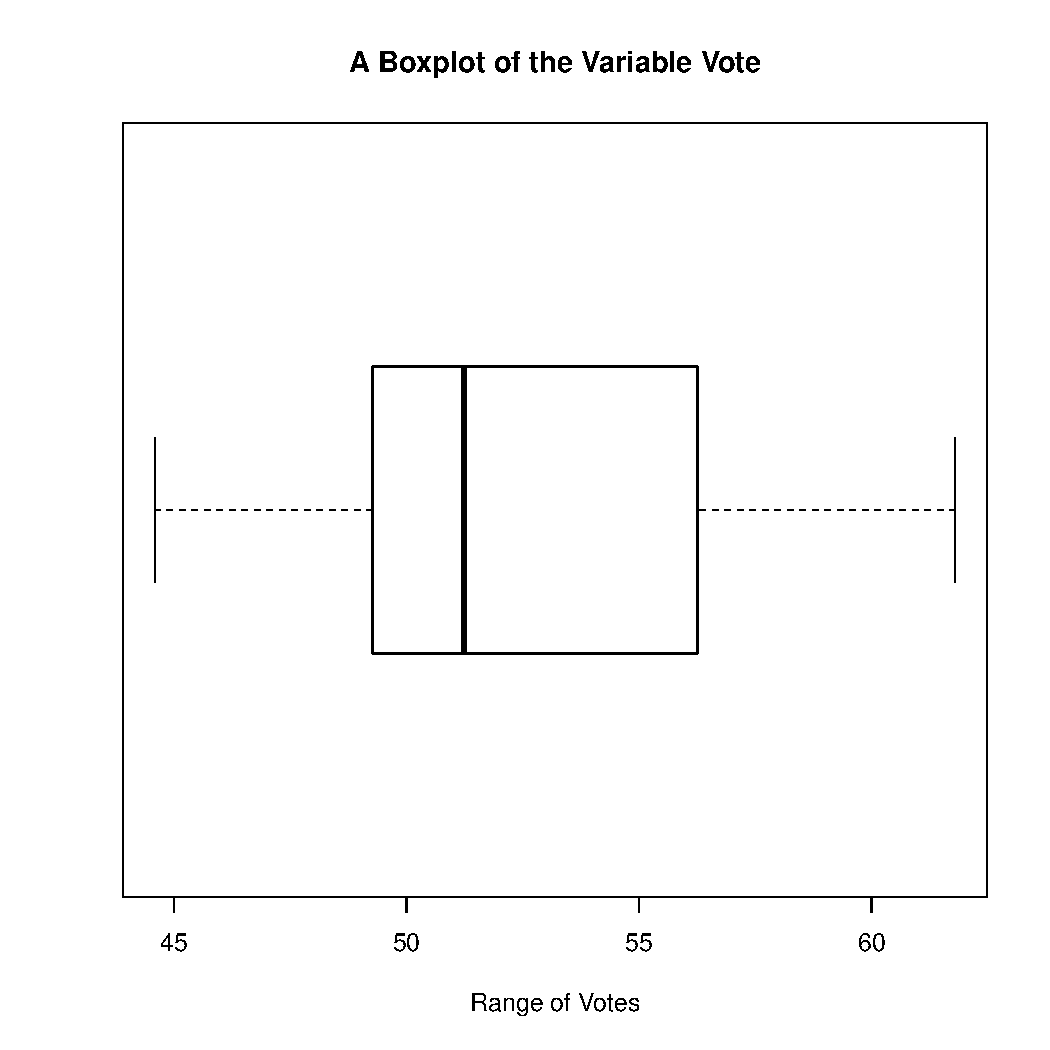
\includegraphics[width=0.9\textwidth]{box1.pdf} 
%     \caption{Boxplot of Incumbent Vote share} % Creates caption underneath graph
%   \end{figure}


% Now all we need to answer the question is a neat table. The easiest way to get a nice looking table is to browse to http://www.tablesgenerator.com. Generate your table just like in Word or any other WYSIWYG editor. Then copy and include the code here. I already did that for you.

% \begin{table}[H]
% \centering
% \begin{tabular}{llllllll}
% \multicolumn{1}{c}{\textbf{Variable}} & \multicolumn{1}{c}{\textit{Mean}} & \multicolumn{1}{c}{\textit{Median}} & \textit{Mode} & \textit{Var} & \textit{SD} & \textit{Range} & \textit{IQR} \\ \hline
% Vote                                  & x                                 & x                                   & x             & x            & x           & x              & x            \\
% Growth                                & x                                 & x                                   & x             & x            & x           & x              & x           
% \end{tabular}
% \caption{Measures of central tendency and variability.}
% \label{my-label}
% \end{table}
% You just have to exchange the x for the right value.

\end{document}
